\section{eo\-Breed$<$ EOT $>$ Class Template Reference}
\label{classeo_breed}\index{eoBreed@{eoBreed}}
Breeding: combination of selecting and transforming a population.  


{\tt \#include $<$eo\-Breed.h$>$}

Inheritance diagram for eo\-Breed$<$ EOT $>$::\begin{figure}[H]
\begin{center}
\leavevmode
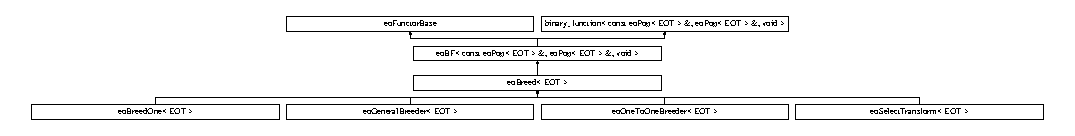
\includegraphics[height=1.37592cm]{classeo_breed}
\end{center}
\end{figure}


\subsection{Detailed Description}
\subsubsection*{template$<$class EOT$>$ class eo\-Breed$<$ EOT $>$}

Breeding: combination of selecting and transforming a population. 

Breeding is thought of a combination of selecting and transforming a population. For efficiency reasons you might want to build your own eo\-Breed derived class rather than relying on a seperate select and transform function.

\begin{Desc}
\item[See also:]{\bf eo\-Select}{\rm (p.\,\pageref{classeo_select})}, {\bf eo\-Transform}{\rm (p.\,\pageref{classeo_transform})}, {\bf eo\-Select\-Transform}{\rm (p.\,\pageref{classeo_select_transform})} \end{Desc}




Definition at line 46 of file eo\-Breed.h.

The documentation for this class was generated from the following file:\begin{CompactItemize}
\item 
eo\-Breed.h\end{CompactItemize}
